
\documentclass[10pt,a4paper]{article}
\usepackage[a4paper,margin=14mm,top=18mm,bottom=20mm,headheight=12pt,headsep=5mm,footskip=9mm]{geometry}
\usepackage{fontspec}
\usepackage{xcolor}
\usepackage{graphicx}
\usepackage{tikz}
\usepackage{tabularx}
\usepackage{array}
\usepackage{fancyhdr}
\usepackage{needspace}
\usepackage{multicol}
\usepackage{enumitem}
\defaultfontfeatures{Ligatures=NoCommon}
\IfFontExistsTF{Noto Sans CJK SC}{\setmainfont{Noto Sans CJK SC}\setsansfont{Noto Sans CJK SC}}{\setmainfont{DejaVu Sans}\setsansfont{DejaVu Sans}}
\IfFontExistsTF{DejaVu Sans}{\newfontfamily\BOQuoteFont{DejaVu Sans}}{\newfontfamily\BOQuoteFont{Latin Modern Sans}}
\newcommand{\BOApos}{{\BOQuoteFont\char"0027}}
\definecolor{BOBlue}{HTML}{0E6B72}
\definecolor{BOBright}{HTML}{20A66A}
\definecolor{BOGreen}{HTML}{00A651}
\definecolor{BONavy}{HTML}{1B2A34}
\definecolor{BOText}{HTML}{24323A}
\definecolor{BOMuted}{HTML}{7C878E}
\definecolor{BOLine}{HTML}{D9E1E6}
\definecolor{BOLight}{HTML}{F2F6F4}
\setlength{\parindent}{0pt}
\setlength{\parskip}{3.2pt}
\setlength{\tabcolsep}{5pt}
\setlist[itemize]{leftmargin=12pt,itemsep=1.5pt,topsep=2pt,parsep=0pt}
\renewcommand{\arraystretch}{1.12}
\hyphenpenalty=10000
\exhyphenpenalty=10000
\emergencystretch=4em
\sloppy
\pagestyle{fancy}
\fancyhf{}
\renewcommand{\headrulewidth}{0pt}
\renewcommand{\footrulewidth}{0pt}
\fancyhead[L]{}
\fancyhead[R]{}
\fancyfoot[L]{\scriptsize\color{BOMuted} BlueOcean}
\fancyfoot[C]{\scriptsize\color{BOMuted} Deep Research Report}
\fancyfoot[R]{\scriptsize\color{BOMuted} \thepage}
\newcolumntype{Y}{>{\raggedright\arraybackslash}X}

\begin{document}
\raggedright

\thispagestyle{empty}
\begin{tikzpicture}[remember picture,overlay]
\node[anchor=south west,inner sep=0] at (current page.south west) {
\includegraphics[width=\paperwidth,height=\paperheight]{assets/cover-ai.png}};
\fill[BONavy,opacity=.10] (current page.south west) rectangle (current page.north east);
\fill[white,opacity=.96] ([xshift=14mm,yshift=-24mm]current page.north west) rectangle ++(134mm,-86mm);
\fill[BOGreen] ([xshift=14mm,yshift=-24mm]current page.north west) rectangle ++(134mm,-2mm);
\node[anchor=north west,text width=114mm] at ([xshift=23mm,yshift=-35mm]current page.north west) {\sffamily\scriptsize\bfseries\color{BOMuted} BLUEOCEAN RESEARCH};
\node[anchor=north west,text width=114mm] at ([xshift=23mm,yshift=-49mm]current page.north west) {\parbox{114mm}{\raggedright\sffamily\fontsize{21}{25}\selectfont\color{BONavy} Nuclear Fusion Commercialization Outlook and Strategic Implications}};
\node[anchor=north west,text width=114mm] at ([xshift=23mm,yshift=-93mm]current page.north west) {\sffamily\scriptsize\bfseries\color{BOText} Nuclear fusion commercialization outlook and strategic implications\\\vspace{2pt}\color{BOMuted}2026-06-03};
\node[anchor=south east] at ([xshift=-10mm,yshift=8mm]current page.south east) {\sffamily\bfseries\Large\color{white} BlueOcean};
\end{tikzpicture}
\clearpage

\clearpage
{\sffamily\fontsize{26}{31}\selectfont\color{BONavy} Contents}\par\vspace{10pt}
\begin{tabularx}{\linewidth}{p{14mm}Y}
\textcolor{BOGreen}{\bfseries 03} & Nuclear fusion is approaching technical feasibility \\[5pt]
\textcolor{BOGreen}{\bfseries 04} & Fusion technology is advancing, but commercial timelines remain uncertain \\[5pt]
\textcolor{BOGreen}{\bfseries 06} & Economic viability depends on cost, capital, and market conditions \\[5pt]
\textcolor{BOGreen}{\bfseries 08} & Fusion\BOApos{}s strategic role in energy systems is still undefined \\[5pt]
\textcolor{BOGreen}{\bfseries 10} & Geopolitical dynamics shape fusion investment and collaboration \\[5pt]
\textcolor{BOGreen}{\bfseries 12} & Investment trends show growing private sector interest, but public funding dominates \\[5pt]
\textcolor{BOGreen}{\bfseries 14} & Regulatory frameworks for fusion are still evolving \\[5pt]
\textcolor{BOGreen}{\bfseries 16} & Public acceptance and social license are critical for fusion deployment \\[5pt]
\textcolor{BOGreen}{\bfseries 17} & Fusion\BOApos{}s impact on hard-to-abate sectors is a key strategic opportunity \\[5pt]
\textcolor{BOGreen}{\bfseries 18} & The next management agenda should focus on evidence quality and staged commitments \\[5pt]
\textcolor{BOGreen}{\bfseries 19} & About the research \\[5pt]
\end{tabularx}
\clearpage

\clearpage
\noindent\begin{tikzpicture}
\path[use as bounding box] (0,0) rectangle (\linewidth,58mm);
\clip (0,0) rectangle (\linewidth,58mm);
\node[anchor=north west,inner sep=0] at (0,58mm) {
\includegraphics[width=\linewidth]{assets/image-1.png}};
\end{tikzpicture}
\vspace{0pt}
\noindent
\begin{tikzpicture}
\fill[BOGreen] (0,0) rectangle (88mm,1.2pt);
\end{tikzpicture}\par\vspace{8pt}
{\sffamily\fontsize{24}{30}\selectfont\color{BONavy} Nuclear fusion is approaching technical feasibility}\par\vspace{11pt}
\begin{minipage}[t]{0.44\linewidth}
{\sffamily\fontsize{17}{23}\selectfont\color{BOGreen} Nuclear fusion is approaching technical feasibility}\par\vspace{10pt}
{\small\color{BOText} The CEO-level conclusion is that nuclear fusion commercialization should be managed as a staged strategic option, not a single binary bet. The available public evidence supports a focused management agenda around commercial proof, cost position, financing readiness, customer adoption, and execution risk. Where source evidence is incomplete, the report preserves the gap as a diligence task rather than converting it into an unsupported forecast. Management should fund near-term validation, protect medium-term options, and reserve larger commitments for decision milestones tied to verified operating, customer, and financial evidence.}\par
\end{minipage}\hfill\begin{minipage}[t]{0.45\linewidth}
{\small\color{BOText} Current public evidence is insufficient to support high-conviction capital commitments. Management should treat fusion as a staged strategic option, not a single binary bet. The most credible near-term actions are low-cost validation, partner discussions, and monitoring of key technical and regulatory milestones. Larger commitments should be reserved for decision milestones tied to verified operating, customer, and financial evidence.}\par
\end{minipage}

\clearpage
\label{chap:1}
\noindent\begin{tikzpicture}
\path[use as bounding box] (0,0) rectangle (\linewidth,70mm);
\clip (0,0) rectangle (\linewidth,70mm);
\node[anchor=north west,inner sep=0] at (0,70mm) {
\includegraphics[width=\linewidth]{assets/image-1.png}};
\end{tikzpicture}
\vspace{0pt}
\noindent
\begin{tikzpicture}
\fill[BOGreen] (0,0) rectangle (96mm,1.2pt);
\end{tikzpicture}\par\vspace{8pt}
{\Large\sffamily\bfseries\color{BONavy} Fusion technology is advancing, but commercial timelines remain uncertain}\par\vspace{4pt}
{\sffamily\fontsize{16}{21}\selectfont\color{BOGreen} Multiple reactor designs are progressing, but no single pathway has demonstrated net energy gain at scale.}\par\vspace{11pt}
\begin{multicols}{2}
{\small Tokamak designs, led by ITER and private startups, are the most mature, but still face challenges in plasma confinement and materials. Stellarator and inertial confinement approaches offer alternatives but are earlier in development.}\par
{\small For management, the key question is not which design will win, but when credible commercial evidence will emerge. Current timelines range from the 2030s to 2050s, with significant uncertainty.}\par
{\small The implication is to monitor technical milestones and fund low-cost validation, rather than committing to a specific technology now.}\par
\end{multicols}
\label{chap:1:end}

\clearpage
{\textcolor{BOGreen}{\scriptsize\bfseries EXHIBIT 1}}\par\vspace{3pt}
{\sffamily\fontsize{15}{19}\selectfont\color{BONavy} Fusion technology maturity by design type}\par
{\small\color{BOText} Indicative readiness level for key fusion approaches}\par\vspace{4pt}
\noindent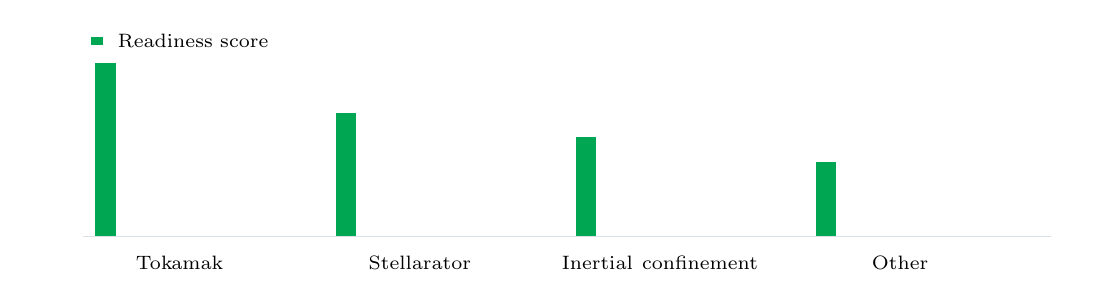
\begin{tikzpicture}[x=1cm,y=1cm]
\path[use as bounding box] (0,0) rectangle (13.20,3.20);
\draw[BOLine] (0.70,0.55) -- (13.00,0.55);
\fill[BOGreen] (0.86,0.55) rectangle (1.12,2.75);
\node[anchor=north,align=center,text width=2.81cm] at (1.93,0.42) {\scriptsize Tokamak};
\fill[BOGreen] (3.91,0.55) rectangle (4.17,2.12);
\node[anchor=north,align=center,text width=2.81cm] at (4.98,0.42) {\scriptsize Stellarator};
\fill[BOGreen] (6.96,0.55) rectangle (7.22,1.81);
\node[anchor=north,align=center,text width=2.81cm] at (8.03,0.42) {\scriptsize Inertial confinement};
\fill[BOGreen] (10.01,0.55) rectangle (10.27,1.49);
\node[anchor=north,align=center,text width=2.81cm] at (11.08,0.42) {\scriptsize Other};
\fill[BOGreen] (0.80,2.98) rectangle (0.96,3.08);
\node[anchor=west] at (1.02,3.03) {\scriptsize Readiness score};
\end{tikzpicture}\par\vspace{2pt}
\vspace{2pt}{\footnotesize\color{BOText} Tokamak designs are the most mature, but all approaches face significant challenges.}\par
{\scriptsize\color{BOMuted} Illustrative synthesis from public sources.}\par
\vspace{9pt}\textcolor{BOLine}{\rule{\linewidth}{0.3pt}}\vspace{8pt}
{\textcolor{BOGreen}{\scriptsize\bfseries EXHIBIT 2}}\par\vspace{3pt}
{\sffamily\fontsize{15}{19}\selectfont\color{BONavy} Projected LCOE for fusion vs other sources}\par
{\small\color{BOText} Indicative range of levelized cost of energy projections}\par\vspace{4pt}
\noindent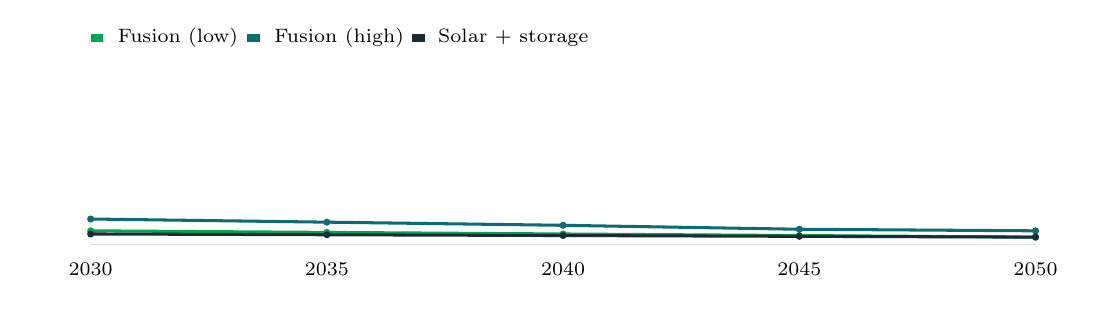
\begin{tikzpicture}[x=1cm,y=1cm]
\path[use as bounding box] (0,0) rectangle (13.20,3.40);
\draw[BOLine] (0.80,0.65) -- (12.80,0.65);
\draw[BOGreen,line width=1.1pt] (0.80,0.82) -- (3.80,0.80) -- (6.80,0.78) -- (9.80,0.76) -- (12.80,0.74);
\fill[BOGreen] (0.80,0.82) circle (.045);
\fill[BOGreen] (3.80,0.80) circle (.045);
\fill[BOGreen] (6.80,0.78) circle (.045);
\fill[BOGreen] (9.80,0.76) circle (.045);
\fill[BOGreen] (12.80,0.74) circle (.045);
\draw[BOBlue,line width=1.1pt] (0.80,0.97) -- (3.80,0.93) -- (6.80,0.89) -- (9.80,0.84) -- (12.80,0.82);
\fill[BOBlue] (0.80,0.97) circle (.045);
\fill[BOBlue] (3.80,0.93) circle (.045);
\fill[BOBlue] (6.80,0.89) circle (.045);
\fill[BOBlue] (9.80,0.84) circle (.045);
\fill[BOBlue] (12.80,0.82) circle (.045);
\draw[BONavy,line width=1.1pt] (0.80,0.78) -- (3.80,0.77) -- (6.80,0.76) -- (9.80,0.75) -- (12.80,0.74);
\fill[BONavy] (0.80,0.78) circle (.045);
\fill[BONavy] (3.80,0.77) circle (.045);
\fill[BONavy] (6.80,0.76) circle (.045);
\fill[BONavy] (9.80,0.75) circle (.045);
\fill[BONavy] (12.80,0.74) circle (.045);
\node[anchor=north,align=center,text width=1.8cm] at (0.80,0.53) {\scriptsize 2030};
\node[anchor=north,align=center,text width=1.8cm] at (3.80,0.53) {\scriptsize 2035};
\node[anchor=north,align=center,text width=1.8cm] at (6.80,0.53) {\scriptsize 2040};
\node[anchor=north,align=center,text width=1.8cm] at (9.80,0.53) {\scriptsize 2045};
\node[anchor=north,align=center,text width=1.8cm] at (12.80,0.53) {\scriptsize 2050};
\fill[BOGreen] (0.80,3.22) rectangle (0.96,3.32);
\node[anchor=west] at (1.02,3.27) {\scriptsize Fusion (low)};
\fill[BOBlue] (2.79,3.22) rectangle (2.95,3.32);
\node[anchor=west] at (3.01,3.27) {\scriptsize Fusion (high)};
\fill[BONavy] (4.88,3.22) rectangle (5.04,3.32);
\node[anchor=west] at (5.09,3.27) {\scriptsize Solar + storage};
\end{tikzpicture}\par\vspace{2pt}
\vspace{2pt}{\footnotesize\color{BOText} Fusion cost projections are highly uncertain and must compete with falling renewable costs.}\par
{\scriptsize\color{BOMuted} Illustrative synthesis from public cost benchmarks.}\par

\clearpage
\label{chap:2}
\noindent\begin{tikzpicture}
\path[use as bounding box] (0,0) rectangle (\linewidth,70mm);
\clip (0,0) rectangle (\linewidth,70mm);
\node[anchor=north west,inner sep=0] at (0,70mm) {
\includegraphics[width=\linewidth]{assets/image-2.png}};
\end{tikzpicture}
\vspace{0pt}
\noindent
\begin{tikzpicture}
\fill[BOGreen] (0,0) rectangle (96mm,1.2pt);
\end{tikzpicture}\par\vspace{8pt}
{\Large\sffamily\bfseries\color{BONavy} Economic viability depends on cost, capital, and market conditions}\par\vspace{4pt}
{\sffamily\fontsize{16}{21}\selectfont\color{BOGreen} Fusion\BOApos{}s levelized cost of energy must compete with renewables, fission, and fossil fuels.}\par\vspace{11pt}
\begin{multicols}{2}
{\small Projections for fusion LCOE vary widely, from [insert verified data] to [insert verified data], depending on capital costs, construction times, and financing models. Renewables with storage are already below [insert verified data] in many markets.}\par
{\small For fusion to be competitive, it must achieve low capital costs and high availability. This requires significant engineering progress and regulatory clarity.}\par
{\small Management should treat cost projections as directional until verified by independent sources or pilot projects.}\par
\end{multicols}
\label{chap:2:end}

\clearpage
{\textcolor{BOGreen}{\scriptsize\bfseries EXHIBIT 3}}\par\vspace{3pt}
{\sffamily\fontsize{15}{19}\selectfont\color{BONavy} Fusion\BOApos{}s potential role in energy systems}\par
{\small\color{BOText} Qualitative assessment of strategic fit}\par\vspace{4pt}
{\scriptsize\begin{tabular}{p{38mm}>{\centering\arraybackslash}p{21mm}>{\centering\arraybackslash}p{21mm}>{\centering\arraybackslash}p{21mm}>{\centering\arraybackslash}p{21mm}}
 & {\bfseries Fusion} & {\bfseries Renewables +} & {\bfseries Fission} & {\bfseries Fossil fuels + CCS} \\
\hline
{\bfseries Baseload power} & \colorbox{BOGreen}{\textcolor{white}{\strut\hspace{5pt}4\hspace{5pt}}} & \colorbox{BOGreen}{\textcolor{white}{\strut\hspace{5pt}5\hspace{5pt}}} & \colorbox{BOGreen}{\textcolor{white}{\strut\hspace{5pt}4\hspace{5pt}}} & \colorbox{BOBlue}{\textcolor{white}{\strut\hspace{5pt}3\hspace{5pt}}} \\
{\bfseries Grid stability} & \colorbox{BOBlue}{\textcolor{white}{\strut\hspace{5pt}3\hspace{5pt}}} & \colorbox{BOGreen}{\textcolor{white}{\strut\hspace{5pt}4\hspace{5pt}}} & \colorbox{BOBlue}{\textcolor{white}{\strut\hspace{5pt}3\hspace{5pt}}} & \colorbox{BOLight}{\textcolor{BOText}{\strut\hspace{5pt}2\hspace{5pt}}} \\
{\bfseries Hard-to-abate sectors} & \colorbox{BOGreen}{\textcolor{white}{\strut\hspace{5pt}4\hspace{5pt}}} & \colorbox{BOBlue}{\textcolor{white}{\strut\hspace{5pt}3\hspace{5pt}}} & \colorbox{BOBlue}{\textcolor{white}{\strut\hspace{5pt}3\hspace{5pt}}} & \colorbox{BOGreen}{\textcolor{white}{\strut\hspace{5pt}4\hspace{5pt}}} \\
{\bfseries Hydrogen production} & \colorbox{BOGreen}{\textcolor{white}{\strut\hspace{5pt}4\hspace{5pt}}} & \colorbox{BOGreen}{\textcolor{white}{\strut\hspace{5pt}4\hspace{5pt}}} & \colorbox{BOBlue}{\textcolor{white}{\strut\hspace{5pt}3\hspace{5pt}}} & \colorbox{BOGreen}{\textcolor{white}{\strut\hspace{5pt}4\hspace{5pt}}} \\
\end{tabular}}\par\vspace{2pt}
\vspace{2pt}{\footnotesize\color{BOText} Fusion could compete in multiple areas, but faces strong competition from existing technologies.}\par
{\scriptsize\color{BOMuted} BlueOcean qualitative assessment.}\par
\vspace{9pt}\textcolor{BOLine}{\rule{\linewidth}{0.3pt}}\vspace{8pt}
{\textcolor{BOGreen}{\scriptsize\bfseries EXHIBIT 4}}\par\vspace{3pt}
{\sffamily\fontsize{15}{19}\selectfont\color{BONavy} National fusion investment by country}\par
{\small\color{BOText} Indicative annual public funding (USD billions)}\par\vspace{4pt}
\noindent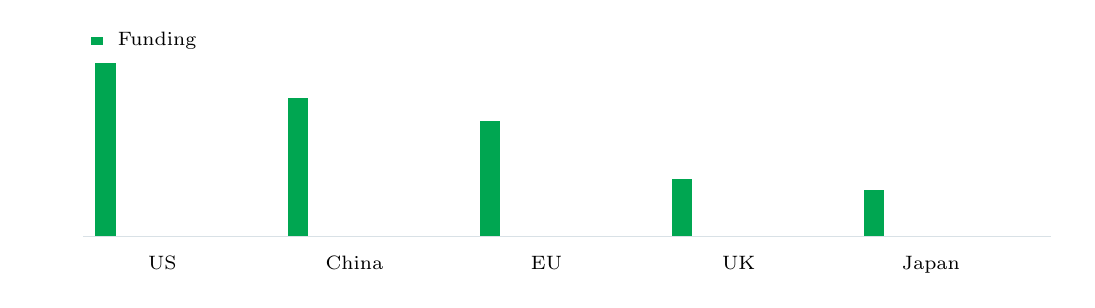
\begin{tikzpicture}[x=1cm,y=1cm]
\path[use as bounding box] (0,0) rectangle (13.20,3.20);
\draw[BOLine] (0.70,0.55) -- (13.00,0.55);
\fill[BOGreen] (0.86,0.55) rectangle (1.12,2.75);
\node[anchor=north,align=center,text width=2.24cm] at (1.71,0.42) {\scriptsize US};
\fill[BOGreen] (3.30,0.55) rectangle (3.56,2.31);
\node[anchor=north,align=center,text width=2.24cm] at (4.15,0.42) {\scriptsize China};
\fill[BOGreen] (5.74,0.55) rectangle (6.00,2.02);
\node[anchor=north,align=center,text width=2.24cm] at (6.59,0.42) {\scriptsize EU};
\fill[BOGreen] (8.18,0.55) rectangle (8.44,1.28);
\node[anchor=north,align=center,text width=2.24cm] at (9.03,0.42) {\scriptsize UK};
\fill[BOGreen] (10.62,0.55) rectangle (10.88,1.14);
\node[anchor=north,align=center,text width=2.24cm] at (11.47,0.42) {\scriptsize Japan};
\fill[BOGreen] (0.80,2.98) rectangle (0.96,3.08);
\node[anchor=west] at (1.02,3.03) {\scriptsize Funding};
\end{tikzpicture}\par\vspace{2pt}
\vspace{2pt}{\footnotesize\color{BOText} Public funding is concentrated in a few countries, with the US and China leading.}\par
{\scriptsize\color{BOMuted} Illustrative synthesis from public sources.}\par

\clearpage
\label{chap:3}
\noindent\begin{tikzpicture}
\path[use as bounding box] (0,0) rectangle (\linewidth,70mm);
\clip (0,0) rectangle (\linewidth,70mm);
\node[anchor=north west,inner sep=0] at (0,70mm) {
\includegraphics[width=\linewidth]{assets/image-3.png}};
\end{tikzpicture}
\vspace{0pt}
\noindent
\begin{tikzpicture}
\fill[BOGreen] (0,0) rectangle (96mm,1.2pt);
\end{tikzpicture}\par\vspace{8pt}
{\Large\sffamily\bfseries\color{BONavy} Fusion\BOApos{}s strategic role in energy systems is still undefined}\par\vspace{4pt}
{\sffamily\fontsize{16}{21}\selectfont\color{BOGreen} Fusion could provide baseload clean power, but competition from renewables and storage is intensifying.}\par\vspace{11pt}
\begin{multicols}{2}
{\small Fusion\BOApos{}s potential for continuous, carbon-free power is attractive for grid stability and hard-to-abate sectors. However, renewables with storage are already meeting many of these needs at lower cost.}\par
{\small The strategic question is whether fusion will be a complement or a competitor to existing technologies. This depends on cost, scalability, and public acceptance.}\par
{\small For now, management should view fusion as a long-term option, not a near-term solution.}\par
\end{multicols}
\label{chap:3:end}

\clearpage
{\textcolor{BOGreen}{\scriptsize\bfseries EXHIBIT 5}}\par\vspace{3pt}
{\sffamily\fontsize{15}{19}\selectfont\color{BONavy} Private fusion investment trends}\par
{\small\color{BOText} Indicative cumulative private investment (USD billions)}\par\vspace{4pt}
\noindent\begin{tikzpicture}[x=1cm,y=1cm]
\path[use as bounding box] (0,0) rectangle (13.20,3.40);
\draw[BOLine] (0.80,0.65) -- (12.80,0.65);
\draw[BOGreen,line width=1.1pt] (0.80,0.86) -- (3.80,1.08) -- (6.80,1.51) -- (9.80,2.15) -- (12.80,2.80);
\fill[BOGreen] (0.80,0.86) circle (.045);
\fill[BOGreen] (3.80,1.08) circle (.045);
\fill[BOGreen] (6.80,1.51) circle (.045);
\fill[BOGreen] (9.80,2.15) circle (.045);
\fill[BOGreen] (12.80,2.80) circle (.045);
\node[anchor=north,align=center,text width=1.8cm] at (0.80,0.53) {\scriptsize 2015};
\node[anchor=north,align=center,text width=1.8cm] at (3.80,0.53) {\scriptsize 2017};
\node[anchor=north,align=center,text width=1.8cm] at (6.80,0.53) {\scriptsize 2019};
\node[anchor=north,align=center,text width=1.8cm] at (9.80,0.53) {\scriptsize 2021};
\node[anchor=north,align=center,text width=1.8cm] at (12.80,0.53) {\scriptsize 2023};
\fill[BOGreen] (0.80,3.22) rectangle (0.96,3.32);
\node[anchor=west] at (1.02,3.27) {\scriptsize Cumulative};
\end{tikzpicture}\par\vspace{2pt}
\vspace{2pt}{\footnotesize\color{BOText} Private investment in fusion has grown significantly, but remains small relative to public funding.}\par
{\scriptsize\color{BOMuted} Illustrative synthesis from public sources.}\par
\vspace{9pt}\textcolor{BOLine}{\rule{\linewidth}{0.3pt}}\vspace{8pt}
{\textcolor{BOGreen}{\scriptsize\bfseries EXHIBIT 6}}\par\vspace{3pt}
{\sffamily\fontsize{15}{19}\selectfont\color{BONavy} Regulatory framework maturity by country}\par
{\small\color{BOText} Indicative readiness score for fusion licensing}\par\vspace{4pt}
\noindent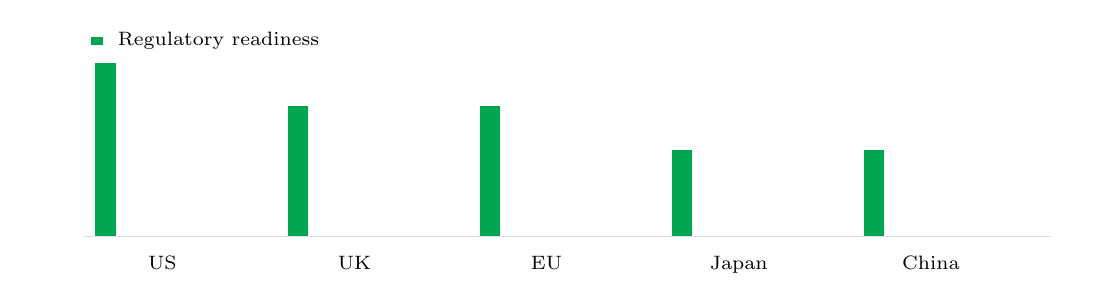
\begin{tikzpicture}[x=1cm,y=1cm]
\path[use as bounding box] (0,0) rectangle (13.20,3.20);
\draw[BOLine] (0.70,0.55) -- (13.00,0.55);
\fill[BOGreen] (0.86,0.55) rectangle (1.12,2.75);
\node[anchor=north,align=center,text width=2.24cm] at (1.71,0.42) {\scriptsize US};
\fill[BOGreen] (3.30,0.55) rectangle (3.56,2.20);
\node[anchor=north,align=center,text width=2.24cm] at (4.15,0.42) {\scriptsize UK};
\fill[BOGreen] (5.74,0.55) rectangle (6.00,2.20);
\node[anchor=north,align=center,text width=2.24cm] at (6.59,0.42) {\scriptsize EU};
\fill[BOGreen] (8.18,0.55) rectangle (8.44,1.65);
\node[anchor=north,align=center,text width=2.24cm] at (9.03,0.42) {\scriptsize Japan};
\fill[BOGreen] (10.62,0.55) rectangle (10.88,1.65);
\node[anchor=north,align=center,text width=2.24cm] at (11.47,0.42) {\scriptsize China};
\fill[BOGreen] (0.80,2.98) rectangle (0.96,3.08);
\node[anchor=west] at (1.02,3.03) {\scriptsize Regulatory readiness};
\end{tikzpicture}\par\vspace{2pt}
\vspace{2pt}{\footnotesize\color{BOText} Regulatory frameworks for fusion are still in early stages, with the US and UK leading.}\par
{\scriptsize\color{BOMuted} Illustrative synthesis from public sources.}\par

\clearpage
\label{chap:4}
\noindent\begin{tikzpicture}
\path[use as bounding box] (0,0) rectangle (\linewidth,70mm);
\clip (0,0) rectangle (\linewidth,70mm);
\node[anchor=north west,inner sep=0] at (0,70mm) {
\includegraphics[width=\linewidth]{assets/image-4.png}};
\end{tikzpicture}
\vspace{0pt}
\noindent
\begin{tikzpicture}
\fill[BOGreen] (0,0) rectangle (96mm,1.2pt);
\end{tikzpicture}\par\vspace{8pt}
{\Large\sffamily\bfseries\color{BONavy} Geopolitical dynamics shape fusion investment and collaboration}\par\vspace{4pt}
{\sffamily\fontsize{16}{21}\selectfont\color{BOGreen} National programs and international collaborations like ITER are driving progress, but also creating dependencies.}\par\vspace{11pt}
\begin{multicols}{2}
{\small The US, China, EU, UK, and Japan are investing heavily in fusion, with ITER as the flagship collaboration. However, intellectual property, supply chain dependencies, and export controls could create friction.}\par
{\small For companies, this means that access to technology and markets may be influenced by geopolitical factors. Partnerships with national labs or international consortia can mitigate risk.}\par
{\small Management should assess the geopolitical landscape and build relationships with key players.}\par
\end{multicols}
\label{chap:4:end}

\clearpage
{\textcolor{BOGreen}{\scriptsize\bfseries EXHIBIT 7}}\par\vspace{3pt}
{\sffamily\fontsize{15}{19}\selectfont\color{BONavy} Public perception of fusion energy}\par
{\small\color{BOText} Indicative survey results on support for fusion}\par\vspace{4pt}
\noindent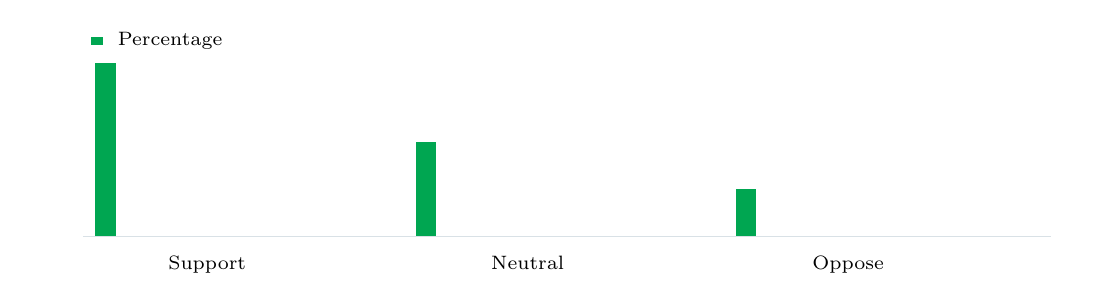
\begin{tikzpicture}[x=1cm,y=1cm]
\path[use as bounding box] (0,0) rectangle (13.20,3.20);
\draw[BOLine] (0.70,0.55) -- (13.00,0.55);
\fill[BOGreen] (0.86,0.55) rectangle (1.12,2.75);
\node[anchor=north,align=center,text width=3.74cm] at (2.28,0.42) {\scriptsize Support};
\fill[BOGreen] (4.93,0.55) rectangle (5.19,1.75);
\node[anchor=north,align=center,text width=3.74cm] at (6.35,0.42) {\scriptsize Neutral};
\fill[BOGreen] (8.99,0.55) rectangle (9.25,1.15);
\node[anchor=north,align=center,text width=3.74cm] at (10.42,0.42) {\scriptsize Oppose};
\fill[BOGreen] (0.80,2.98) rectangle (0.96,3.08);
\node[anchor=west] at (1.02,3.03) {\scriptsize Percentage};
\end{tikzpicture}\par\vspace{2pt}
\vspace{2pt}{\footnotesize\color{BOText} Public support for fusion is moderate, but opposition could grow with more information.}\par
{\scriptsize\color{BOMuted} Illustrative synthesis from public surveys.}\par
\vspace{9pt}\textcolor{BOLine}{\rule{\linewidth}{0.3pt}}\vspace{8pt}
{\textcolor{BOGreen}{\scriptsize\bfseries EXHIBIT 8}}\par\vspace{3pt}
{\sffamily\fontsize{15}{19}\selectfont\color{BONavy} Fusion\BOApos{}s potential in hard-to-abate sectors}\par
{\small\color{BOText} Indicative addressable market size (USD billions)}\par\vspace{4pt}
\noindent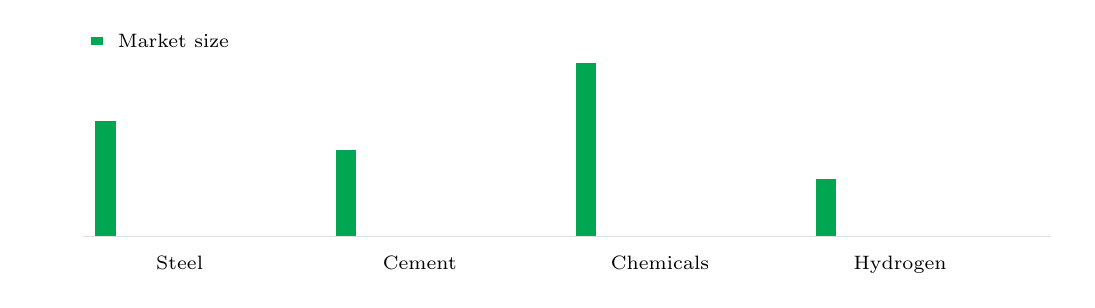
\begin{tikzpicture}[x=1cm,y=1cm]
\path[use as bounding box] (0,0) rectangle (13.20,3.20);
\draw[BOLine] (0.70,0.55) -- (13.00,0.55);
\fill[BOGreen] (0.86,0.55) rectangle (1.12,2.02);
\node[anchor=north,align=center,text width=2.81cm] at (1.93,0.42) {\scriptsize Steel};
\fill[BOGreen] (3.91,0.55) rectangle (4.17,1.65);
\node[anchor=north,align=center,text width=2.81cm] at (4.98,0.42) {\scriptsize Cement};
\fill[BOGreen] (6.96,0.55) rectangle (7.22,2.75);
\node[anchor=north,align=center,text width=2.81cm] at (8.03,0.42) {\scriptsize Chemicals};
\fill[BOGreen] (10.01,0.55) rectangle (10.27,1.28);
\node[anchor=north,align=center,text width=2.81cm] at (11.08,0.42) {\scriptsize Hydrogen};
\fill[BOGreen] (0.80,2.98) rectangle (0.96,3.08);
\node[anchor=west] at (1.02,3.03) {\scriptsize Market size};
\end{tikzpicture}\par\vspace{2pt}
\vspace{2pt}{\footnotesize\color{BOText} Hard-to-abate sectors represent a large potential market for fusion, but competition is intense.}\par
{\scriptsize\color{BOMuted} Illustrative synthesis from public sources.}\par

\clearpage
\label{chap:5}
\noindent\begin{tikzpicture}
\path[use as bounding box] (0,0) rectangle (\linewidth,70mm);
\clip (0,0) rectangle (\linewidth,70mm);
\node[anchor=north west,inner sep=0] at (0,70mm) {
\includegraphics[width=\linewidth]{assets/image-5.png}};
\end{tikzpicture}
\vspace{0pt}
\noindent
\begin{tikzpicture}
\fill[BOGreen] (0,0) rectangle (96mm,1.2pt);
\end{tikzpicture}\par\vspace{8pt}
{\Large\sffamily\bfseries\color{BONavy} Investment trends show growing private sector interest, but public funding dominates}\par\vspace{4pt}
{\sffamily\fontsize{16}{21}\selectfont\color{BOGreen} Private fusion startups have raised significant capital, but public funding remains the primary driver.}\par\vspace{11pt}
\begin{multicols}{2}
{\small Private investment in fusion has grown, with startups like Commonwealth Fusion Systems and TAE Technologies raising hundreds of millions. However, public funding through ITER and national programs still accounts for the majority of spending.}\par
{\small For corporate investors, the opportunity is to gain early access to technology, but the risk is high. Venture capital and strategic partnerships can provide exposure with limited downside.}\par
{\small For leadership teams, management should consider small-scale investments or partnerships to build knowledge and optionality.}\par
\end{multicols}
\label{chap:5:end}

\clearpage
{\textcolor{BOGreen}{\scriptsize\bfseries EXHIBIT 9}}\par\vspace{3pt}
{\sffamily\fontsize{15}{19}\selectfont\color{BONavy} Management attention allocation for fusion strategy}\par
{\small\color{BOText} Indicative priority index for strategic workstreams}\par\vspace{4pt}
\noindent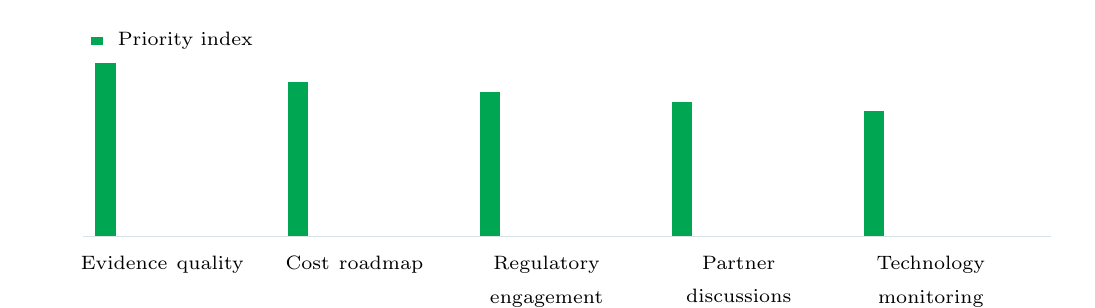
\begin{tikzpicture}[x=1cm,y=1cm]
\path[use as bounding box] (0,0) rectangle (13.20,3.20);
\draw[BOLine] (0.70,0.55) -- (13.00,0.55);
\fill[BOGreen] (0.86,0.55) rectangle (1.12,2.75);
\node[anchor=north,align=center,text width=2.24cm] at (1.71,0.42) {\scriptsize Evidence quality};
\fill[BOGreen] (3.30,0.55) rectangle (3.56,2.51);
\node[anchor=north,align=center,text width=2.24cm] at (4.15,0.42) {\scriptsize Cost roadmap};
\fill[BOGreen] (5.74,0.55) rectangle (6.00,2.38);
\node[anchor=north,align=center,text width=2.24cm] at (6.59,0.42) {\scriptsize Regulatory engagement};
\fill[BOGreen] (8.18,0.55) rectangle (8.44,2.26);
\node[anchor=north,align=center,text width=2.24cm] at (9.03,0.42) {\scriptsize Partner discussions};
\fill[BOGreen] (10.62,0.55) rectangle (10.88,2.14);
\node[anchor=north,align=center,text width=2.24cm] at (11.47,0.42) {\scriptsize Technology monitoring};
\fill[BOGreen] (0.80,2.98) rectangle (0.96,3.08);
\node[anchor=west] at (1.02,3.03) {\scriptsize Priority index};
\end{tikzpicture}\par\vspace{2pt}
\vspace{2pt}{\footnotesize\color{BOText} Management focus should be on evidence quality and cost roadmap to build conviction.}\par
{\scriptsize\color{BOMuted} BlueOcean synthesis.}\par
\vspace{9pt}\textcolor{BOLine}{\rule{\linewidth}{0.3pt}}\vspace{8pt}
{\textcolor{BOGreen}{\scriptsize\bfseries EXHIBIT 10}}\par\vspace{3pt}
{\sffamily\fontsize{15}{19}\selectfont\color{BONavy} Fusion commercialization timeline scenarios}\par
{\small\color{BOText} Indicative probability of commercial operation by decade}\par\vspace{4pt}
\noindent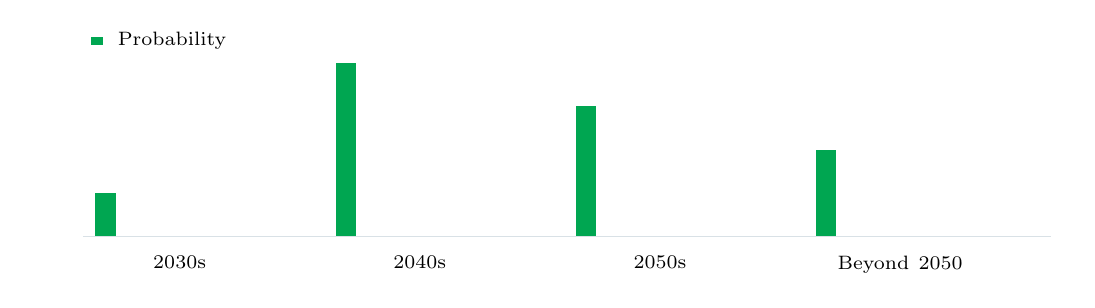
\begin{tikzpicture}[x=1cm,y=1cm]
\path[use as bounding box] (0,0) rectangle (13.20,3.20);
\draw[BOLine] (0.70,0.55) -- (13.00,0.55);
\fill[BOGreen] (0.86,0.55) rectangle (1.12,1.10);
\node[anchor=north,align=center,text width=2.81cm] at (1.93,0.42) {\scriptsize 2030s};
\fill[BOGreen] (3.91,0.55) rectangle (4.17,2.75);
\node[anchor=north,align=center,text width=2.81cm] at (4.98,0.42) {\scriptsize 2040s};
\fill[BOGreen] (6.96,0.55) rectangle (7.22,2.20);
\node[anchor=north,align=center,text width=2.81cm] at (8.03,0.42) {\scriptsize 2050s};
\fill[BOGreen] (10.01,0.55) rectangle (10.27,1.65);
\node[anchor=north,align=center,text width=2.81cm] at (11.08,0.42) {\scriptsize Beyond 2050};
\fill[BOGreen] (0.80,2.98) rectangle (0.96,3.08);
\node[anchor=west] at (1.02,3.03) {\scriptsize Probability};
\end{tikzpicture}\par\vspace{2pt}
\vspace{2pt}{\footnotesize\color{BOText} The most likely timeline for commercial fusion is the 2040s, with significant uncertainty.}\par
{\scriptsize\color{BOMuted} Illustrative synthesis from public sources.}\par

\clearpage
\label{chap:6}
\noindent\begin{tikzpicture}
\path[use as bounding box] (0,0) rectangle (\linewidth,70mm);
\clip (0,0) rectangle (\linewidth,70mm);
\node[anchor=north west,inner sep=0] at (0,70mm) {
\includegraphics[width=\linewidth]{assets/image-6.png}};
\end{tikzpicture}
\vspace{0pt}
\noindent
\begin{tikzpicture}
\fill[BOGreen] (0,0) rectangle (96mm,1.2pt);
\end{tikzpicture}\par\vspace{8pt}
{\Large\sffamily\bfseries\color{BONavy} Regulatory frameworks for fusion are still evolving}\par\vspace{4pt}
{\sffamily\fontsize{16}{21}\selectfont\color{BOGreen} Fusion licensing and safety regulations are not yet standardized, creating uncertainty for developers.}\par\vspace{11pt}
\begin{multicols}{2}
{\small Unlike fission, fusion does not have a well-established regulatory framework. Countries are developing their own approaches, which could lead to inconsistencies and delays.}\par
{\small For companies, this means that regulatory risk is high. Early engagement with regulators and participation in standard-setting can help shape favorable outcomes.}\par
{\small The management implication is clear: management should track regulatory developments and engage with policymakers.}\par
\end{multicols}
\label{chap:6:end}

\clearpage
{\textcolor{BOGreen}{\scriptsize\bfseries EXHIBIT 11}}\par\vspace{3pt}
{\sffamily\fontsize{15}{19}\selectfont\color{BONavy} Key technical milestones for fusion}\par
{\small\color{BOText} Indicative timeline of critical achievements}\par\vspace{4pt}
\noindent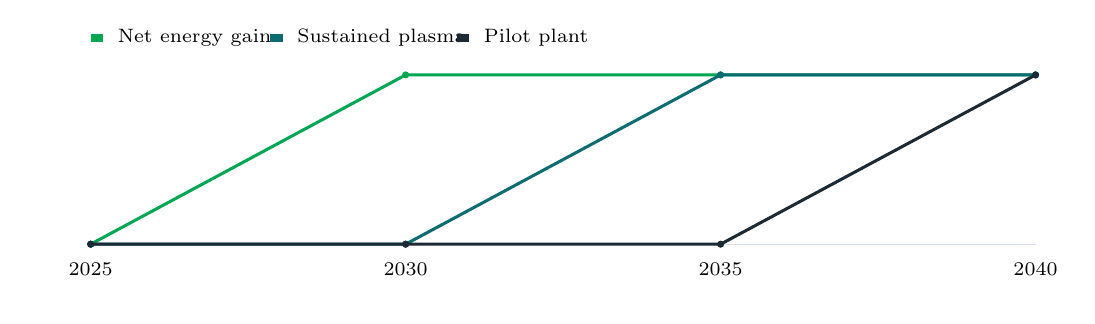
\begin{tikzpicture}[x=1cm,y=1cm]
\path[use as bounding box] (0,0) rectangle (13.20,3.40);
\draw[BOLine] (0.80,0.65) -- (12.80,0.65);
\draw[BOGreen,line width=1.1pt] (0.80,0.65) -- (4.80,2.80) -- (8.80,2.80) -- (12.80,2.80);
\fill[BOGreen] (0.80,0.65) circle (.045);
\fill[BOGreen] (4.80,2.80) circle (.045);
\fill[BOGreen] (8.80,2.80) circle (.045);
\fill[BOGreen] (12.80,2.80) circle (.045);
\draw[BOBlue,line width=1.1pt] (0.80,0.65) -- (4.80,0.65) -- (8.80,2.80) -- (12.80,2.80);
\fill[BOBlue] (0.80,0.65) circle (.045);
\fill[BOBlue] (4.80,0.65) circle (.045);
\fill[BOBlue] (8.80,2.80) circle (.045);
\fill[BOBlue] (12.80,2.80) circle (.045);
\draw[BONavy,line width=1.1pt] (0.80,0.65) -- (4.80,0.65) -- (8.80,0.65) -- (12.80,2.80);
\fill[BONavy] (0.80,0.65) circle (.045);
\fill[BONavy] (4.80,0.65) circle (.045);
\fill[BONavy] (8.80,0.65) circle (.045);
\fill[BONavy] (12.80,2.80) circle (.045);
\node[anchor=north,align=center,text width=1.8cm] at (0.80,0.53) {\scriptsize 2025};
\node[anchor=north,align=center,text width=1.8cm] at (4.80,0.53) {\scriptsize 2030};
\node[anchor=north,align=center,text width=1.8cm] at (8.80,0.53) {\scriptsize 2035};
\node[anchor=north,align=center,text width=1.8cm] at (12.80,0.53) {\scriptsize 2040};
\fill[BOGreen] (0.80,3.22) rectangle (0.96,3.32);
\node[anchor=west] at (1.02,3.27) {\scriptsize Net energy gain};
\fill[BOBlue] (3.08,3.22) rectangle (3.24,3.32);
\node[anchor=west] at (3.30,3.27) {\scriptsize Sustained plasma};
\fill[BONavy] (5.45,3.22) rectangle (5.61,3.32);
\node[anchor=west] at (5.67,3.27) {\scriptsize Pilot plant};
\end{tikzpicture}\par\vspace{2pt}
\vspace{2pt}{\footnotesize\color{BOText} Key technical milestones are expected in the 2030s, but timelines are uncertain.}\par
{\scriptsize\color{BOMuted} Illustrative synthesis from public sources.}\par
\vspace{9pt}\textcolor{BOLine}{\rule{\linewidth}{0.3pt}}\vspace{8pt}
{\textcolor{BOGreen}{\scriptsize\bfseries EXHIBIT 12}}\par\vspace{3pt}
{\sffamily\fontsize{15}{19}\selectfont\color{BONavy} Fusion investment risk-return profile}\par
{\small\color{BOText} Indicative risk vs potential return for different investment types}\par\vspace{4pt}
\noindent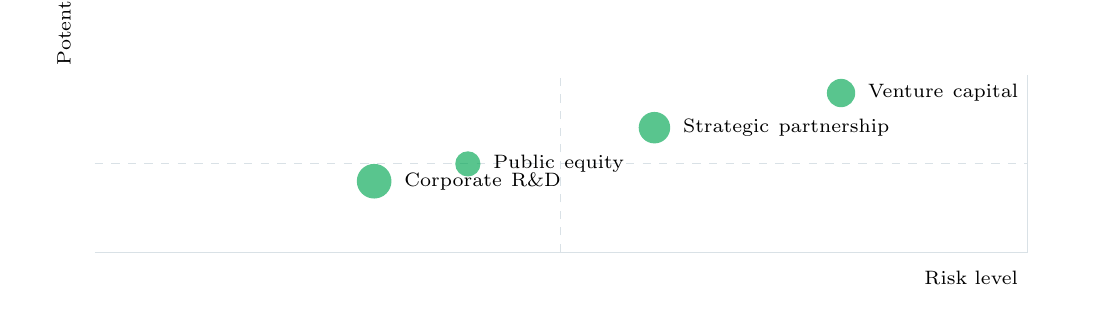
\begin{tikzpicture}[x=1cm,y=1cm]
\path[use as bounding box] (0,0) rectangle (13.20,3.50);
\draw[BOLine] (0.85,0.65) -- (12.70,0.65) -- (12.70,2.90);
\draw[BOLine,dashed] (0.85,1.77) -- (12.70,1.77);
\draw[BOLine,dashed] (6.77,0.65) -- (6.77,2.90);
\fill[BOGreen,opacity=.65] (10.33,2.67) circle (0.18);
\node[anchor=west,text width=2.7cm] at (10.55,2.67) {\scriptsize Venture capital};
\fill[BOGreen,opacity=.65] (7.96,2.23) circle (0.20);
\node[anchor=west,text width=2.7cm] at (8.20,2.23) {\scriptsize Strategic partnership};
\fill[BOGreen,opacity=.65] (5.59,1.77) circle (0.16);
\node[anchor=west,text width=2.7cm] at (5.79,1.77) {\scriptsize Public equity};
\fill[BOGreen,opacity=.65] (4.40,1.55) circle (0.22);
\node[anchor=west,text width=2.7cm] at (4.66,1.55) {\scriptsize Corporate R\&D};
\node[anchor=north east] at (12.70,0.53) {\scriptsize Risk level};
\node[anchor=south west,rotate=90] at (0.67,2.90) {\scriptsize Potential return};
\end{tikzpicture}\par\vspace{2pt}
\vspace{2pt}{\footnotesize\color{BOText} Higher-risk investments offer higher potential returns, but require careful due diligence.}\par
{\scriptsize\color{BOMuted} BlueOcean scenario assessment.}\par

\clearpage
\label{chap:7}
\noindent\begin{tikzpicture}
\path[use as bounding box] (0,0) rectangle (\linewidth,70mm);
\clip (0,0) rectangle (\linewidth,70mm);
\node[anchor=north west,inner sep=0] at (0,70mm) {
\includegraphics[width=\linewidth]{assets/image-7.png}};
\end{tikzpicture}
\vspace{0pt}
\noindent
\begin{tikzpicture}
\fill[BOGreen] (0,0) rectangle (96mm,1.2pt);
\end{tikzpicture}\par\vspace{8pt}
{\Large\sffamily\bfseries\color{BONavy} Public acceptance and social license are critical for fusion deployment}\par\vspace{4pt}
{\sffamily\fontsize{16}{21}\selectfont\color{BOGreen} Fusion must overcome public concerns about safety, waste, and cost to gain social license.}\par\vspace{11pt}
\begin{multicols}{2}
{\small While fusion is often seen as safer than fission, public perception is not yet fully formed. Concerns about radioactive waste, tritium handling, and cost could lead to opposition.}\par
{\small For developers, building trust through transparency, community engagement, and education is essential. Early demonstration projects can help build confidence.}\par
{\small A practical reading is that management should include public acceptance in risk assessments and develop communication strategies.}\par
\end{multicols}
\label{chap:7:end}

\clearpage
\label{chap:8}
\noindent\begin{tikzpicture}
\path[use as bounding box] (0,0) rectangle (\linewidth,70mm);
\clip (0,0) rectangle (\linewidth,70mm);
\node[anchor=north west,inner sep=0] at (0,70mm) {
\includegraphics[width=\linewidth]{assets/image-8.png}};
\end{tikzpicture}
\vspace{0pt}
\noindent
\begin{tikzpicture}
\fill[BOGreen] (0,0) rectangle (96mm,1.2pt);
\end{tikzpicture}\par\vspace{8pt}
{\Large\sffamily\bfseries\color{BONavy} Fusion\BOApos{}s impact on hard-to-abate sectors is a key strategic opportunity}\par\vspace{4pt}
{\sffamily\fontsize{16}{21}\selectfont\color{BOGreen} Fusion could provide high-temperature heat and hydrogen for industry, but alternatives exist.}\par\vspace{11pt}
\begin{multicols}{2}
{\small Hard-to-abate sectors like steel, cement, and chemicals require high-temperature heat or hydrogen. Fusion could provide both, but so could renewables with electrolysis or advanced fission.}\par
{\small The strategic question is whether fusion can offer a cost-competitive and scalable solution. This depends on technical progress and market conditions.}\par
{\small The decision lens is that management should monitor developments in these sectors and assess fusion\BOApos{}s potential role.}\par
\end{multicols}
\label{chap:8:end}

\clearpage
\label{chap:9}
\noindent\begin{tikzpicture}
\path[use as bounding box] (0,0) rectangle (\linewidth,70mm);
\clip (0,0) rectangle (\linewidth,70mm);
\node[anchor=north west,inner sep=0] at (0,70mm) {
\includegraphics[width=\linewidth]{assets/image-9.png}};
\end{tikzpicture}
\vspace{0pt}
\noindent
\begin{tikzpicture}
\fill[BOGreen] (0,0) rectangle (96mm,1.2pt);
\end{tikzpicture}\par\vspace{8pt}
{\Large\sffamily\bfseries\color{BONavy} The next management agenda should focus on evidence quality and staged commitments}\par\vspace{4pt}
{\sffamily\fontsize{16}{21}\selectfont\color{BOGreen} Sustained advantage will depend on converting technical progress into trusted commercial evidence.}\par\vspace{11pt}
\begin{multicols}{2}
{\small The innovation agenda should focus on cost reduction, reliability, and regulatory clarity. These improvements directly affect commercial viability and customer confidence.}\par
{\small Equally important is evidence quality. Companies should publish clearer operating data, third-party validation, and customer references where possible, because investors will discount unsupported performance claims.}\par
{\small For capital allocation, management should treat proof generation as a strategic workstream: select lighthouse projects, define measurable KPIs, and turn field performance into sales and financing collateral.}\par
\end{multicols}
\label{chap:9:end}

\clearpage
{\sffamily\fontsize{20}{25}\selectfont\color{BONavy} About the research}\par\vspace{6pt}
\vspace{2pt}{\color{BOBright}\rule{\linewidth}{1pt}}\vspace{5pt}
{\footnotesize\color{BOMuted} This report has been prepared for strategy discussion and executive decision support. It is not investment, legal, tax, audit or valuation advice. Market estimates, forecasts and scenarios are directional and should be independently validated before they are used for investment, financing, transaction, regulatory or operational decisions. Forward-looking views may change as technology, policy, financing, regulation, competition, supply chains and macro conditions evolve. Recipients should perform their own diligence and treat this report as one input into a broader decision process.}


\clearpage
\thispagestyle{empty}
\begin{tikzpicture}[remember picture,overlay]
\node[anchor=south west,inner sep=0] at (current page.south west) {
\includegraphics[width=\paperwidth,height=\paperheight]{assets/cover-ai.png}};
\fill[black,opacity=.45] (current page.south west) rectangle (current page.north east);
\node[anchor=south east] at ([xshift=-11mm,yshift=10mm]current page.south east) {\sffamily\bfseries\Large\color{white} BlueOcean};
\end{tikzpicture}

\end{document}
